\documentclass[a4paper,12pt]{article}
\usepackage{fullpage}
\usepackage{amsmath,amsthm,amsfonts,amssymb,amscd}
\usepackage{xcolor}
\usepackage{graphicx}
\usepackage{xepersian}
\usepackage{placeins}

\newcommand{\StudentOne}{4011262134}
\newcommand{\StudentTwo}{4011262098}
\newcommand{\NameOne}{مینا جمشیدی}
\newcommand{\NameTwo}{مبینا محمدی}
\newcommand{\ProjectName}{مستندات پروژه clustering}


\definecolor{CustomBackground}{HTML}{1C1C1C}
\pagecolor{CustomBackground}
\color{white}


\settextfont{Vazir.ttf}[
BoldFont = Vazir-Bold.ttf, 
Path = fonts/]
\setlatintextfont{Vazir.ttf}[
BoldFont = Vazir-Bold.ttf, 
Path = fonts/]


\renewcommand{\baselinestretch}{1.2}
\let\nobreaksection\section
\renewcommand{\section}{\nobreaksection} 

\begin{document}
	

	\hrule \medskip
	\begin{minipage}{0.3\textwidth}
		\raggedright
		\small
		\NameOne \\
		\StudentOne \\
		\NameTwo \\
		\StudentTwo
	\end{minipage}
	\begin{minipage}{0.4\textwidth} 
		\centering 
		\large\bfseries
		\ProjectName \\
	\end{minipage}
	\begin{minipage}{0.3\textwidth}
		\raggedleft
		\small
	\end{minipage}
	\medskip\hrule 
	\vspace*{1.5cm}  
	
\section{نتایج فاز اول: استخراج ویژگی و طبقه‌بندی ابتدایی}


در این بخش، عملکرد مدل‌های طبقه‌بندی مختلف بر پایه سه سطح متفاوت از ویژگی‌های استخراج‌شده از مدل \lr{ResNet18} مورد ارزیابی قرار گرفت. ویژگی‌ها به سه دسته تقسیم شدند: ویژگی‌های سطح پایین (تا لایه \lr{maxpool})، ویژگی‌های میانی (تا پایان \lr{layer2}) و ویژگی‌های سطح بالا (تا لایه \lr{avgpool}). برای هر سطح، شش مدل طبقه‌بندی مختلف شامل \lr{SVM}، \lr{KNN}، \lr{Random Forest}، \lr{Logistic Regression}، \lr{Extra Trees} و \lr{Gaussian NB} آموزش داده شدند و دقت آن‌ها روی مجموعه داده‌ی آزمایشی بررسی شد.

\vspace{0.5cm}
\textbf{۱. ویژگی‌های سطح پایین \lr{(Low-Level Features)}:}

در این سطح، ویژگی‌ها شامل لبه‌ها، الگوهای ابتدایی و اطلاعات بافتی پایه هستند. نتایج نشان دادند که این ویژگی‌ها در تفکیک کلاس‌ها محدودیت دارند. دقت بهترین مدل (\lr{Logistic Regression}) برابر با \lr{71\%} روی داده‌های آزمایشی بود. کلاس \lr{horses} به طور قابل توجهی بهتر از \lr{cats} و \lr{dogs} طبقه‌بندی شد که نشان‌دهنده‌ی تمایز بیشتر این کلاس در ویژگی‌های سطح پایین است.
\begin{figure}[h]
	\centering
	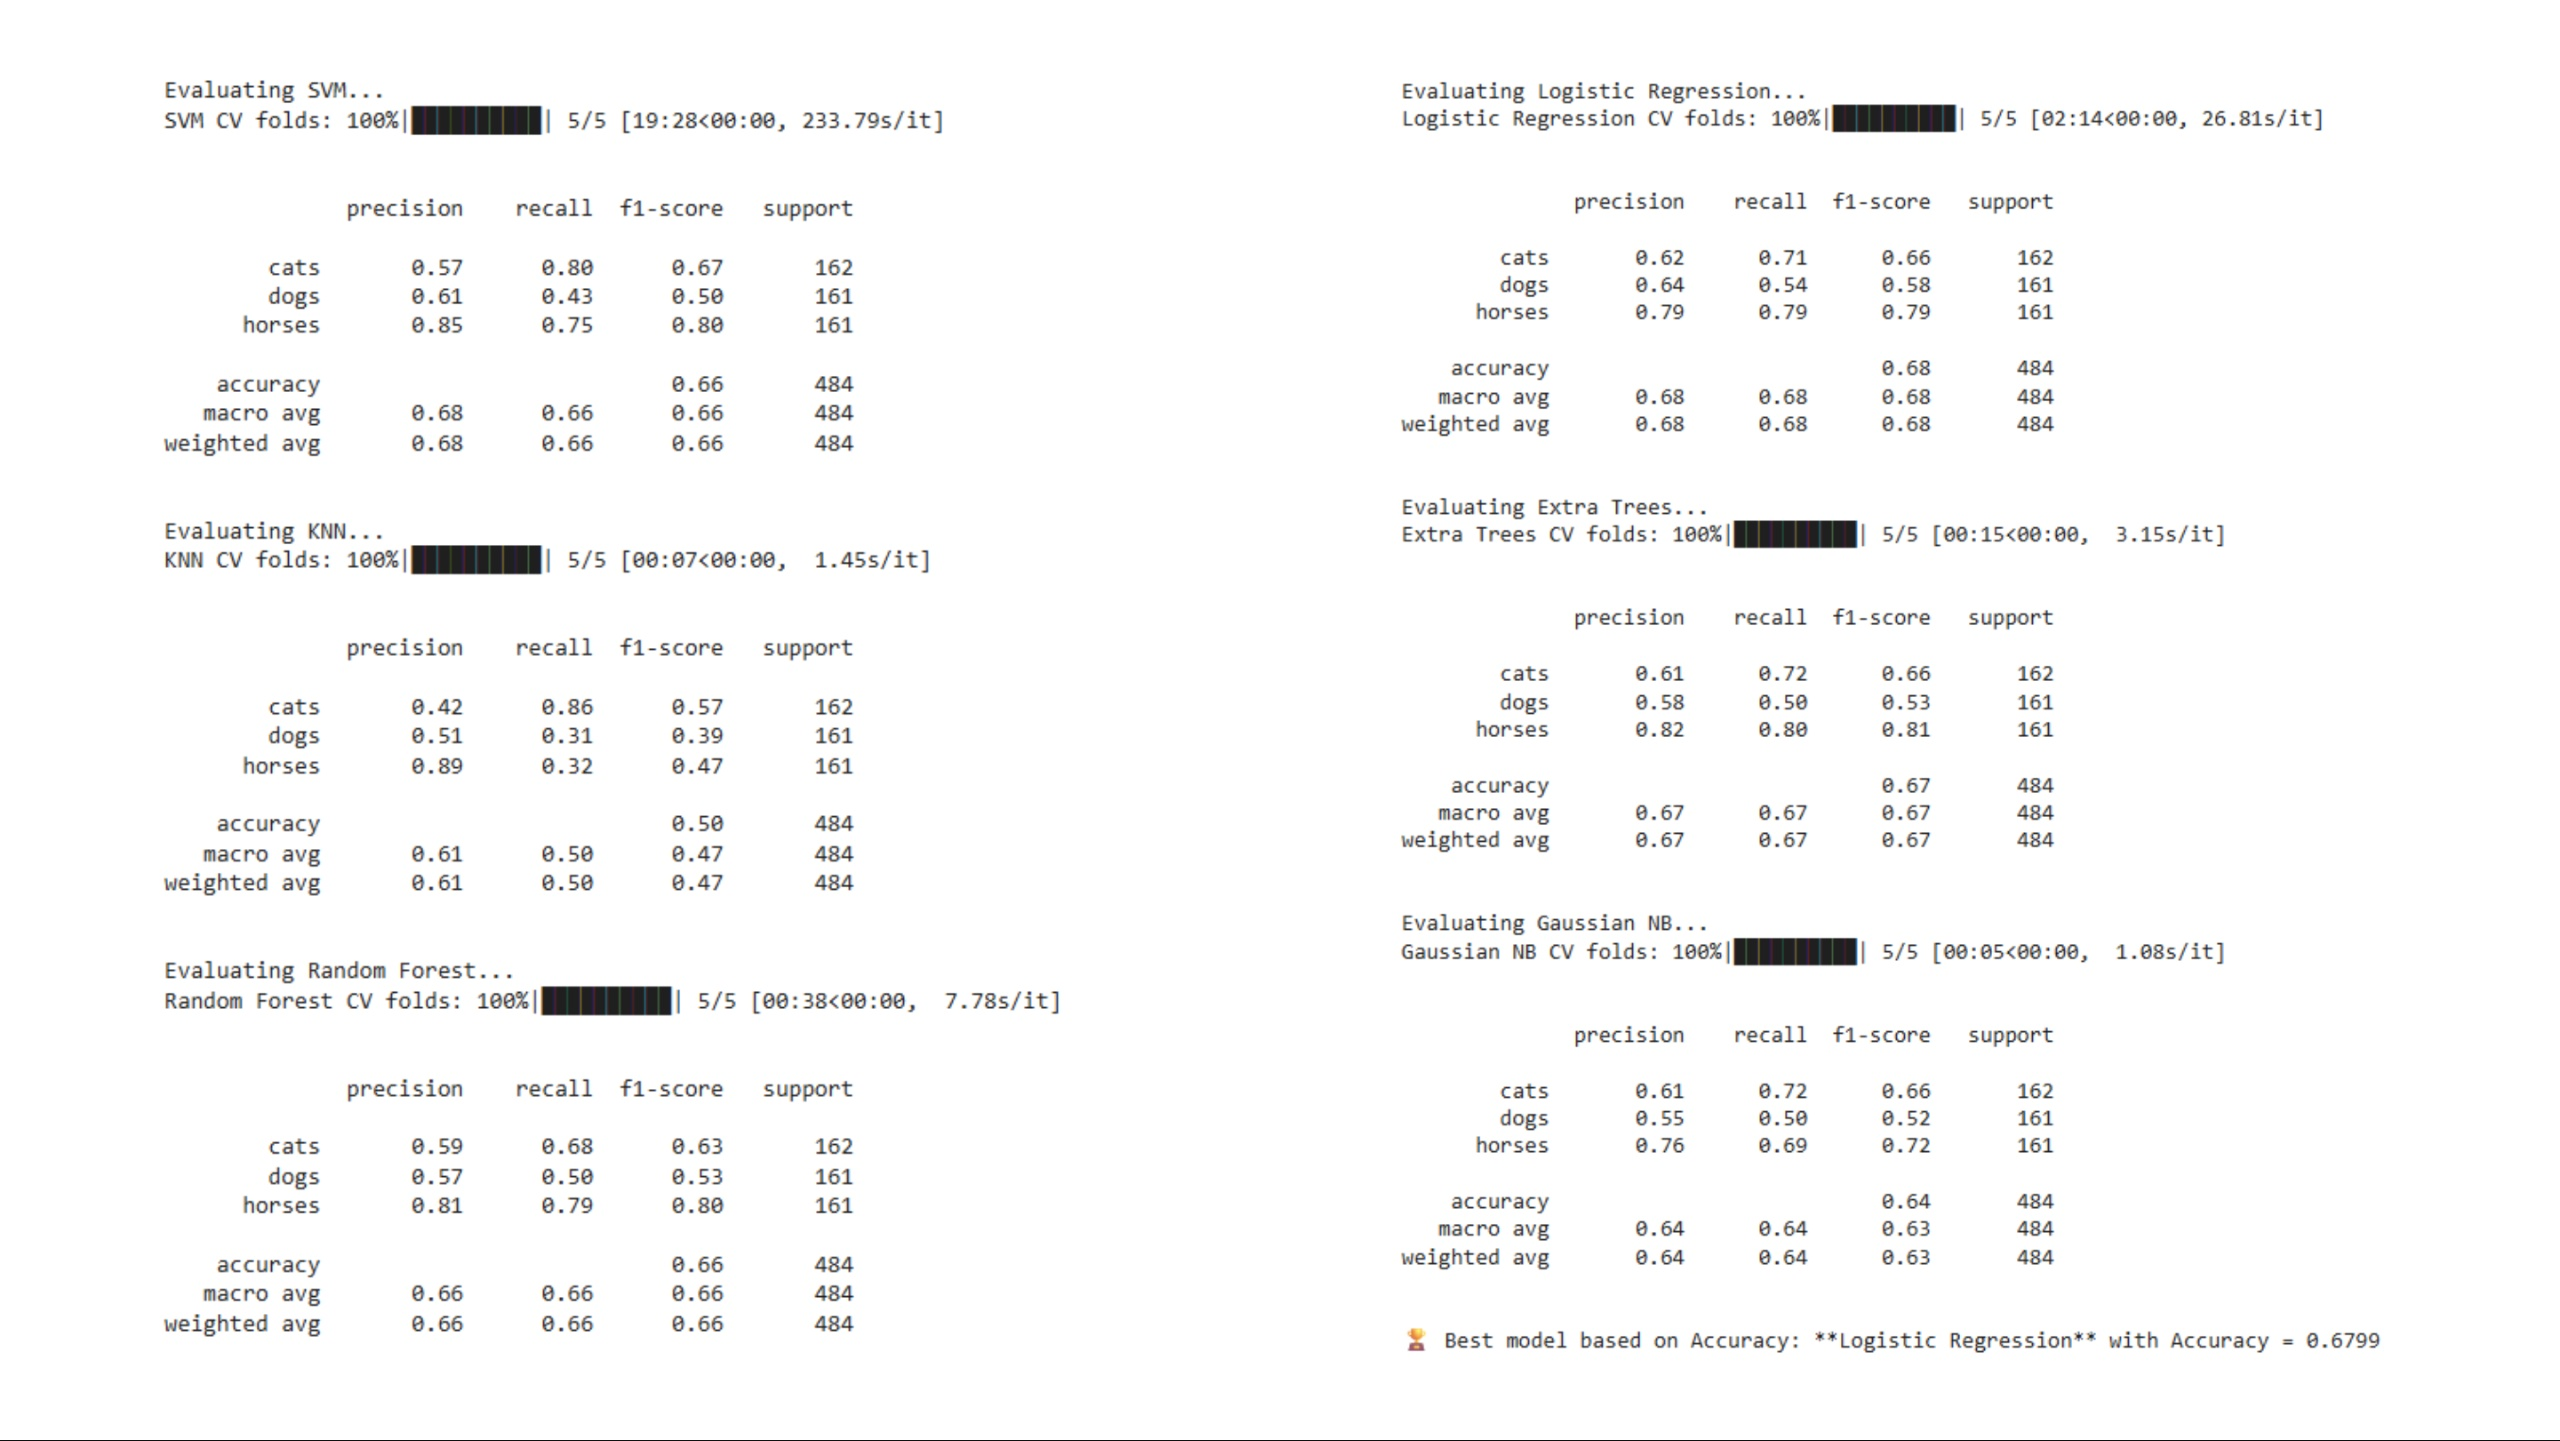
\includegraphics[width=1\textwidth]{1-1.jpg}
\end{figure}
\FloatBarrier
\begin{figure}[h]
	\centering
	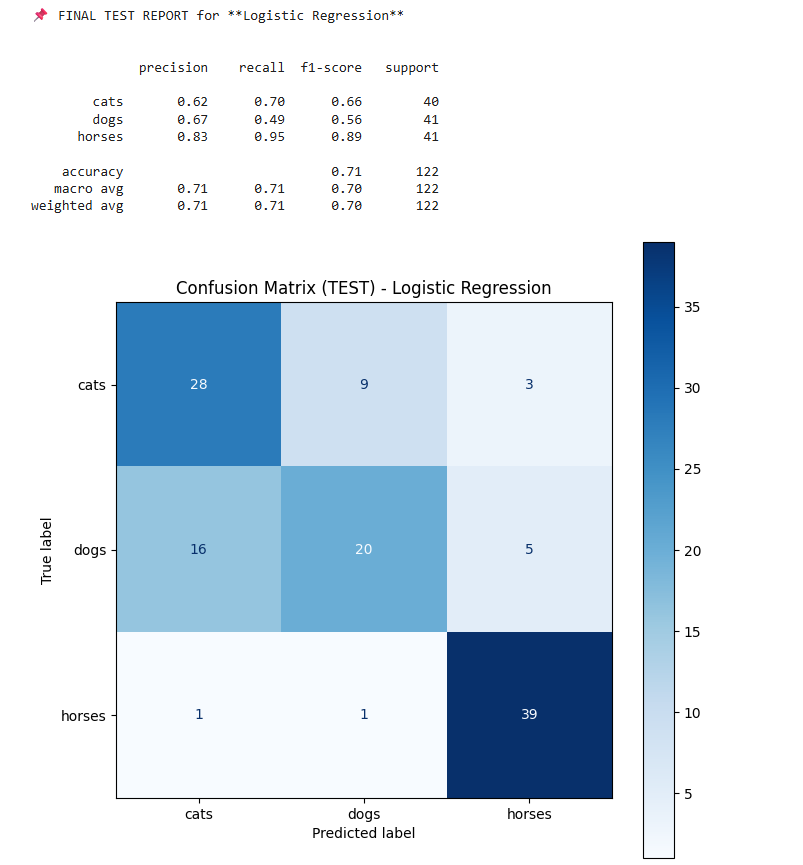
\includegraphics[width=1\textwidth]{1-2.png}
\end{figure}
\FloatBarrier

\textbf{۲. ویژگی‌های میانی \lr{(Mid-Level Features)}:}

با استفاده از لایه‌های \lr{layer1} و \lr{layer2}، مدل قادر به استخراج ویژگی‌های ترکیبی و ساختاریافته‌تری شد. در این مرحله، دقت مدل \lr{Logistic Regression} به حدود \lr{85\%} افزایش یافت و کلاس‌ها به صورت متوازن‌تری طبقه‌بندی شدند. نسبت به مرحله‌ی قبل، کلاس \lr{dogs} که پیش‌تر عملکرد ضعیفی داشت، بهبود محسوسی در دقت و \lr{recall} نشان داد. این موضوع حاکی از قدرت بیشتر ویژگی‌های میانی در بازنمایی ساختارهای مفهومی‌تر تصویر است.

\begin{figure}[h]
	\centering
	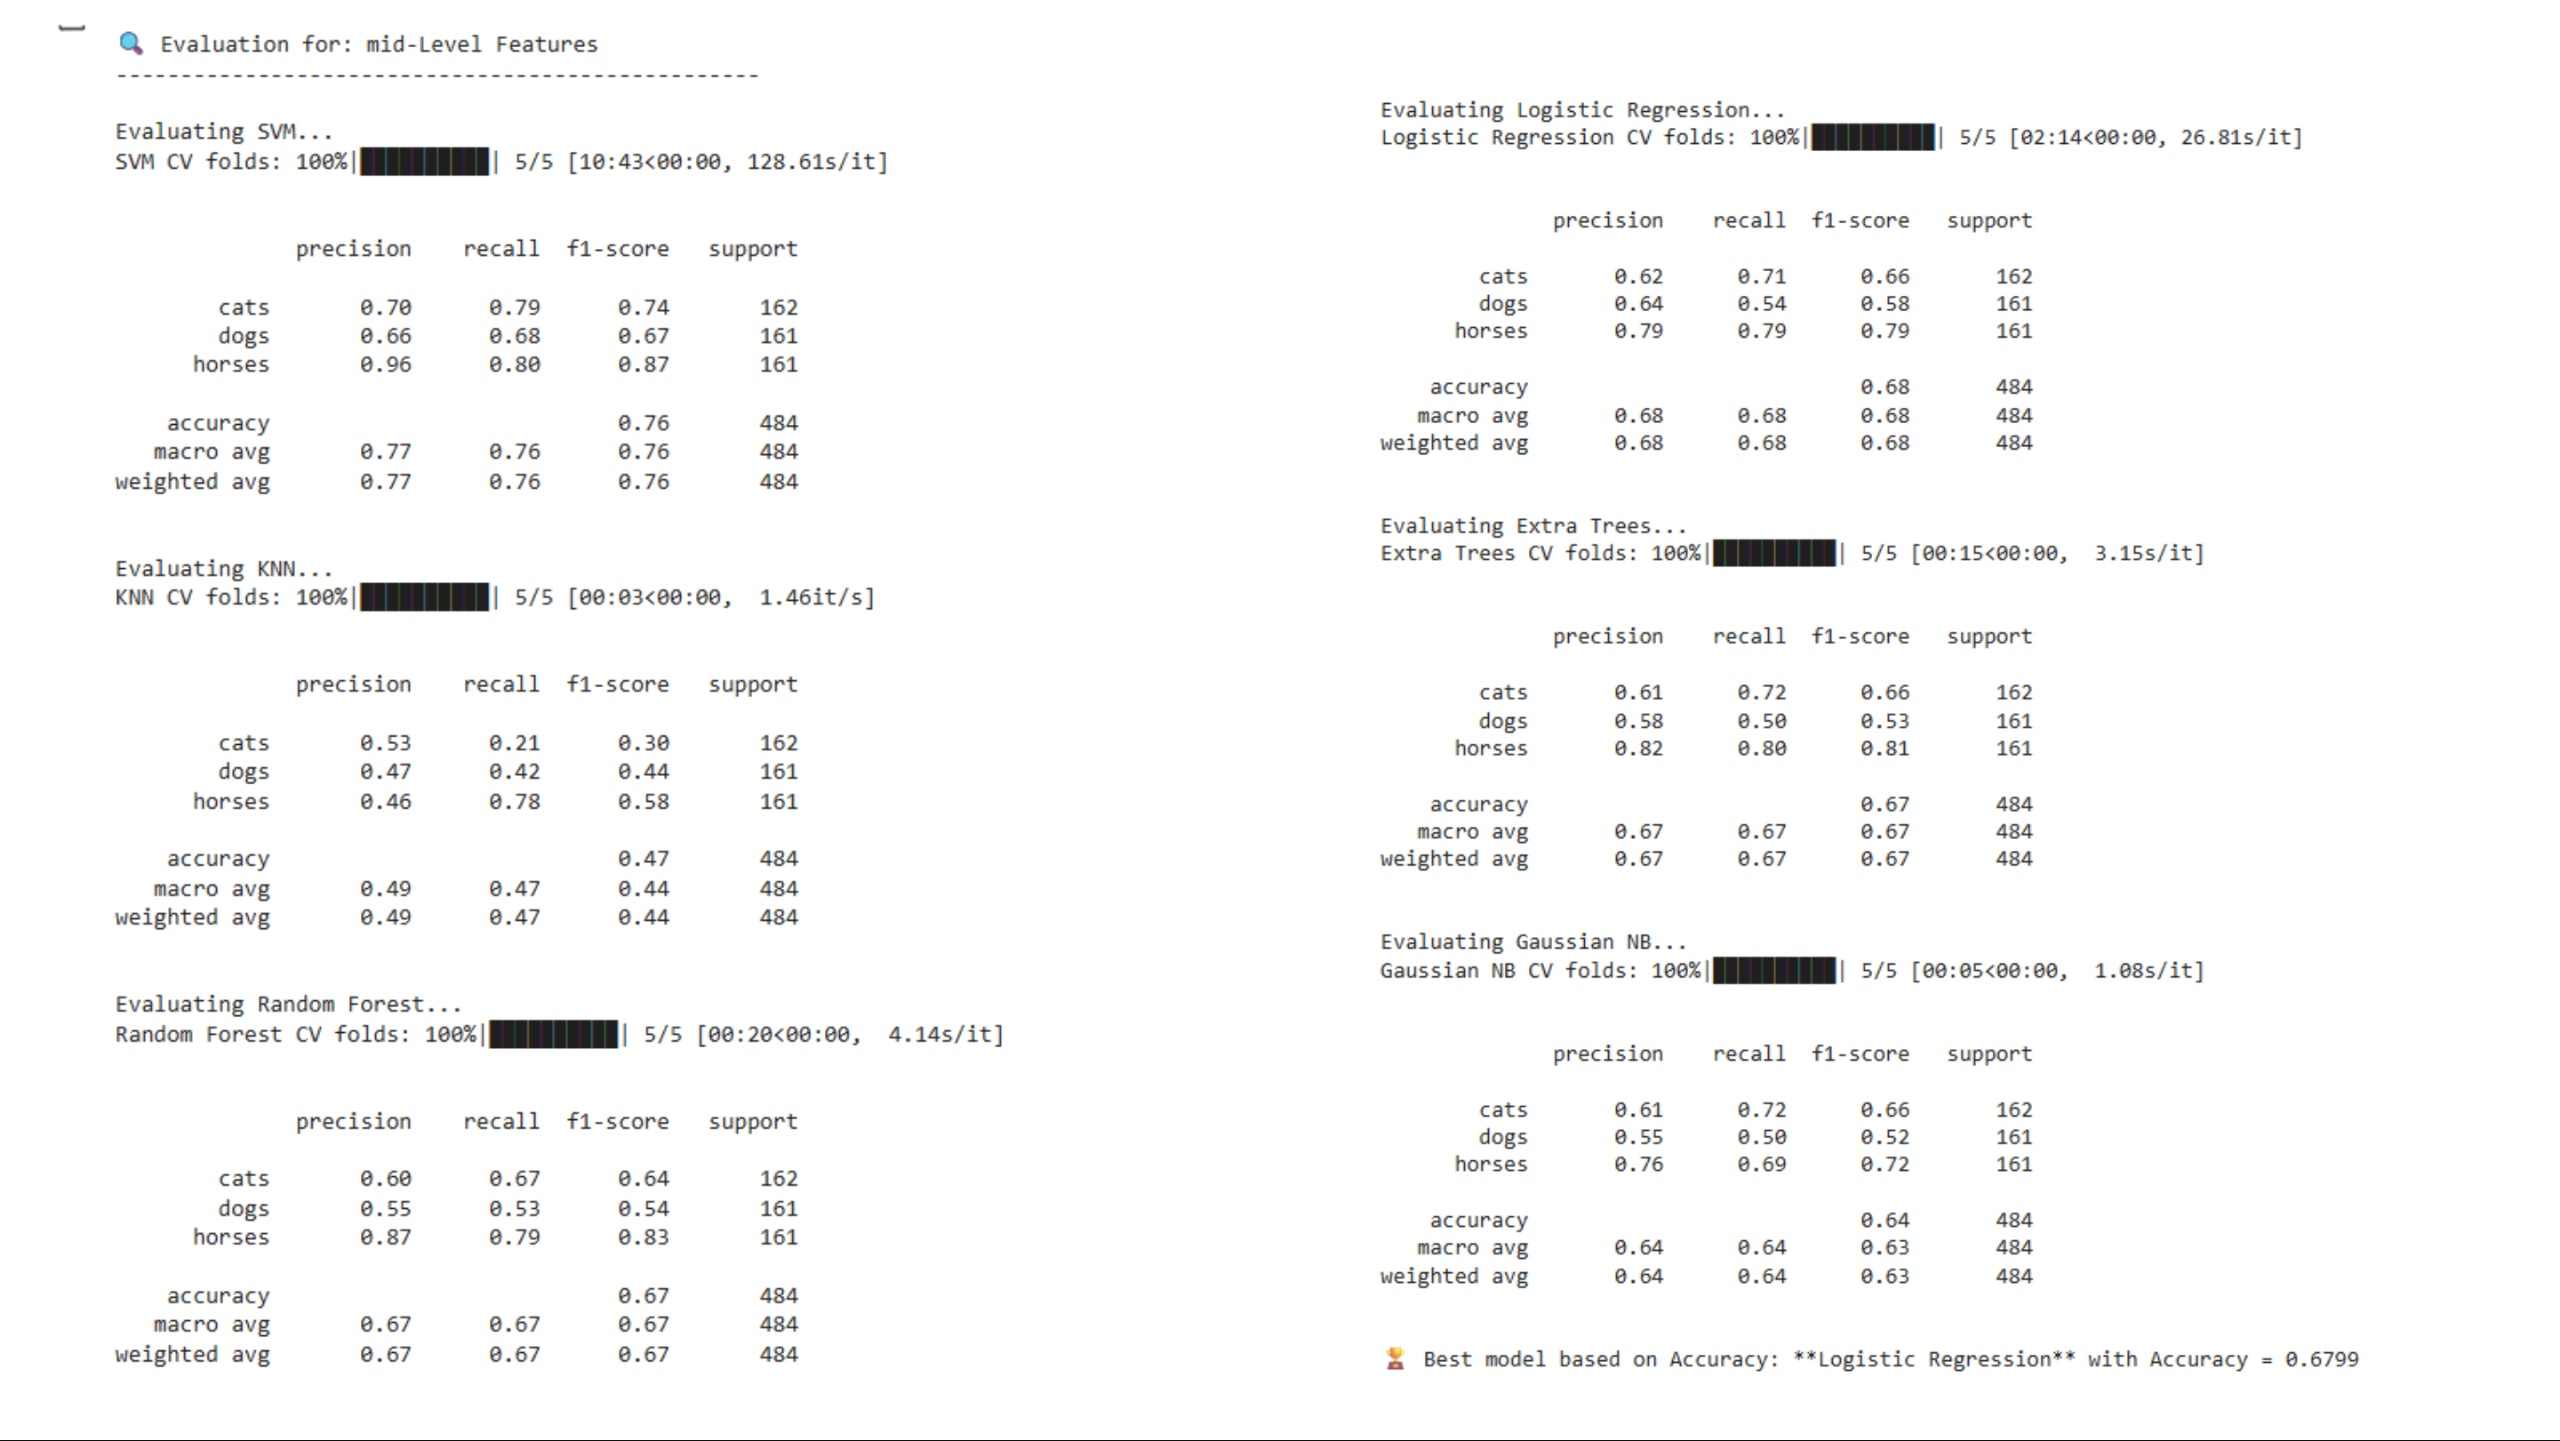
\includegraphics[width=1\textwidth]{2-1.jpg}
\end{figure}
\FloatBarrier
\begin{figure}[h]
	\centering
	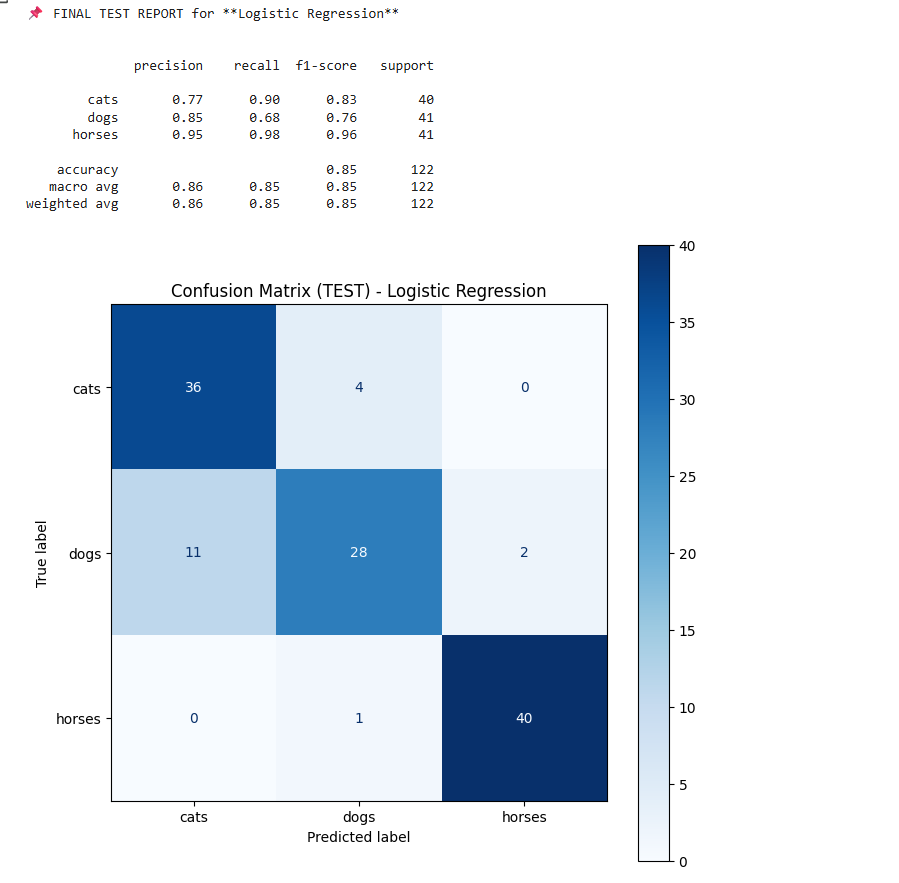
\includegraphics[width=1\textwidth]{2-2.png}
\end{figure}
\FloatBarrier

\textbf{۳. ویژگی‌های سطح بالا \lr{(High-Level Features)}:}

در این حالت، از تمام شبکه (به جز لایه FC نهایی) برای استخراج ویژگی استفاده شد. این ویژگی‌ها شامل نمایش‌های انتزاعی از مفاهیم بصری مانند "چهره گربه" یا "پیکربندی بدن اسب" هستند. مدل \lr{SVM} در این مرحله با دقت \lr{100\%} روی داده‌ی تست بهترین عملکرد را نشان داد. تمامی کلاس‌ها بدون خطا شناسایی شدند. این نتیجه تأییدی بر قدرت بالای نمایش‌های سطح بالا در مدل‌های یادگیری عمیق برای تفکیک دقیق بین کلاس‌ها است.

\begin{figure}[h]
	\centering
	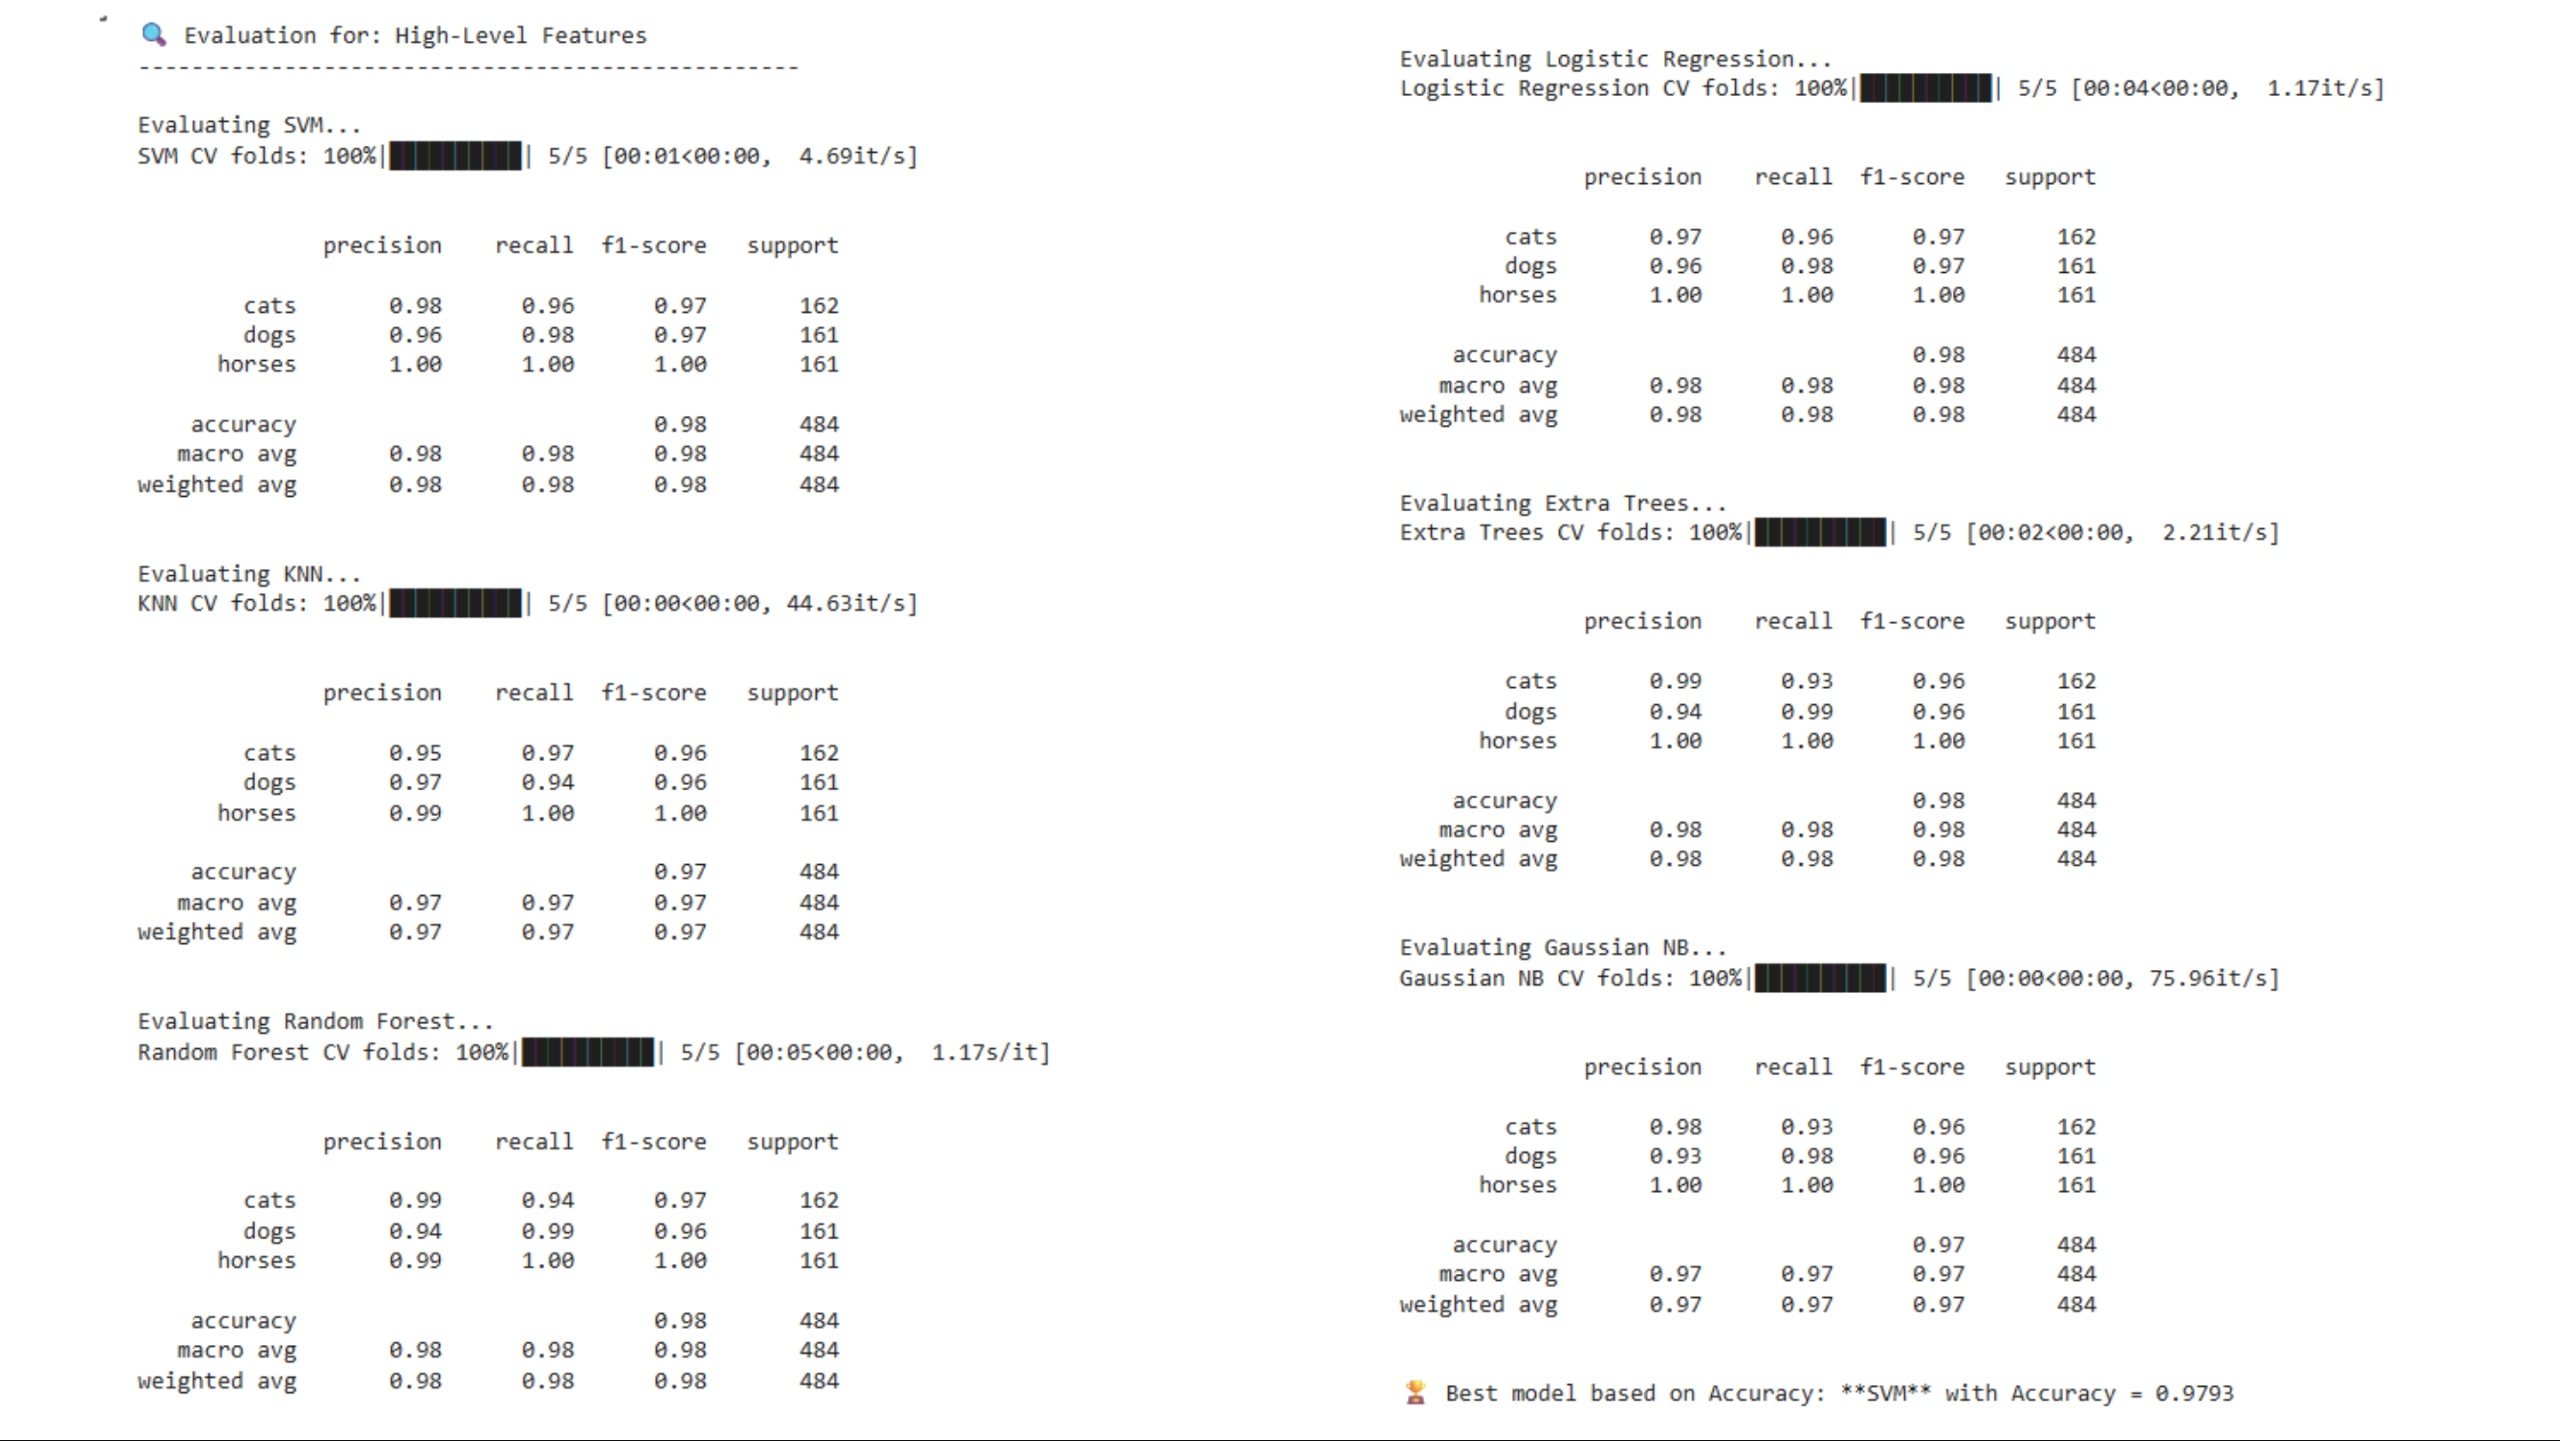
\includegraphics[width=1\textwidth]{3-1.jpg}
\end{figure}
\FloatBarrier
\begin{figure}[h]
	\centering
	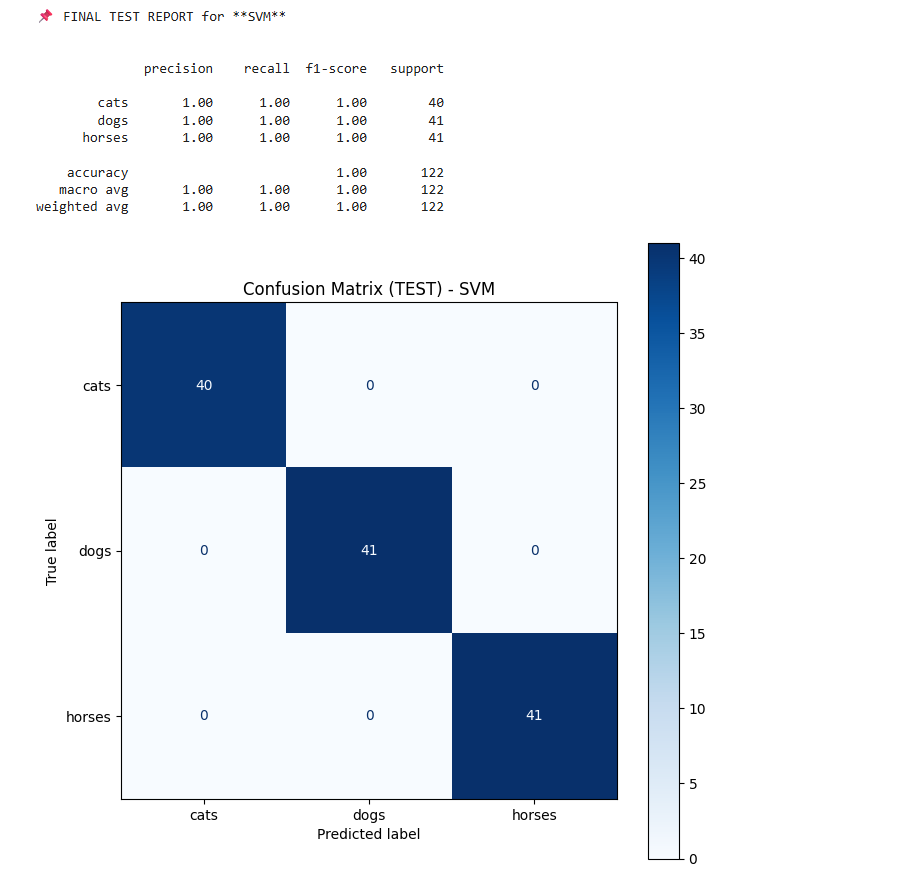
\includegraphics[width=1\textwidth]{3-2.png}
\end{figure}
\FloatBarrier
\vspace{0.5cm}
\textbf{جمع‌بندی:}

\begin{itemize}
	\item با افزایش عمق ویژگی‌های استخراج‌شده، دقت و کیفیت طبقه‌بندی نیز به‌طور قابل توجهی افزایش یافت.
	\item مدل \lr{Logistic Regression} در دو سطح اول بهترین عملکرد را داشت، در حالی که در سطح سوم، مدل \lr{SVM} با اختلاف واضحی بهترین بود.
	\item کلاس \lr{horses} در تمامی سطوح نسبت به دو کلاس دیگر بهتر طبقه‌بندی شد، که می‌تواند به تفاوت‌های بصری بارزتر این کلاس نسبت داده شود.
	\item نتایج نشان می‌دهند که حتی بدون \lr{fine-tuning} شبکه، استفاده از ویژگی‌های استخراج‌شده از \lr{ResNet18} می‌تواند عملکرد بالایی در طبقه‌بندی تصاویر داشته باشد.
\end{itemize}


\end{document}